\section{Compression}

\subsection{Pruning}

  It can be computationally and memory intensive to train and utilize neural networks. This is where network pruning comes in, which attempts to identify a subnetwork that performs as well as the original. Given a neural net $f(\mathbf{x}, \boldsymbol{\theta})$ where $\boldsymbol{\theta} \in \mathbb{R}^M$, a pruned neural network can be thought of as a subnetwork $f(\mathbf{x}, \mathbf{m} \odot \boldsymbol{\theta})$, where $\mathbf{m}$ is a \textbf{mask}, i.e. a vector in $\{0, 1\}^M$ that, when multiplied component-wise to $\boldsymbol{\theta}$, essentially ``deletes" a portion of the parameters. 

  \begin{center}
    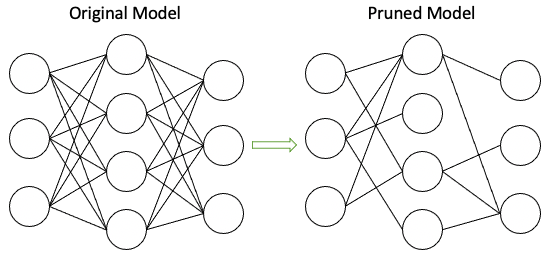
\includegraphics[scale=0.4]{img/pruned_network.png}
  \end{center}

  This idea has been around for a long time, and the general method of pruning is as such: 
  \begin{enumerate}
      \item We initialize the neural network $f(\mathbf{x}, \boldsymbol{\theta}_0)$ and train it until we have $f(\mathbf{x}, \boldsymbol{\theta})$. 
      \item We now prune the network. The most basic pruning scheme is to keep the top $k\%$ largest weights, since smaller weights do not contribute much to the forward prop, and thus can be ignored. 
  \end{enumerate}
  These pruned networks have been shown to reach accuracies as high as the original network, with equal training progress. Now, if we were to take only this pruned network and train it from the beginning, it will perform as well as the original network, \textit{only under} the condition that we start from the same initialization $\mathbf{m} \odot \boldsymbol{\theta}$. If we take this subnetwork and initialize it differently at $\boldsymbol{\theta}_0^\prime$, then this subnetwork would not train well. Therefore, the performance of the pruned network is dependent on the initialization! 

  If we had initialized the full network differently, trained it, and then pruned again, we may have a different subnetwork that will only train well on its own given this new initialization. Therefore, a good initialization is extremely important for training subnetworks. This fact doesn't help much since we can't just take some arbitrary subnetwork and train it since we don't know the good initialization. We must always train the full network, then find the subnetwork, and then find its initialization. 

  This is essentially the \textbf{lottery ticket hypothesis} \cite{lottery}, which states that a randomly-initialized, dense neural network contains a subnetwork that is initialized such that, when trained in isolation, it can match the test accuracy of the original network after training for at must the same number of iterations. 

  This paper hints at why neural networks work at all. It first states that only a very small subnetwork is responsible for the vast majority of its performance, but it must be initialized at the right position. But by overparameterizing these neural nets so much (by a certain margin), they have so many different combinations of subnetworks such that whatever initialization you throw at it, it is guaranteed that some subnetwork within it will train well with this initialization. This subnetwork is called the \textit{winning ticket}. 

\subsection{Quantization}

